\documentclass{article}
\usepackage{tikz}
\usetikzlibrary{positioning,arrows,calc}
\begin{document}
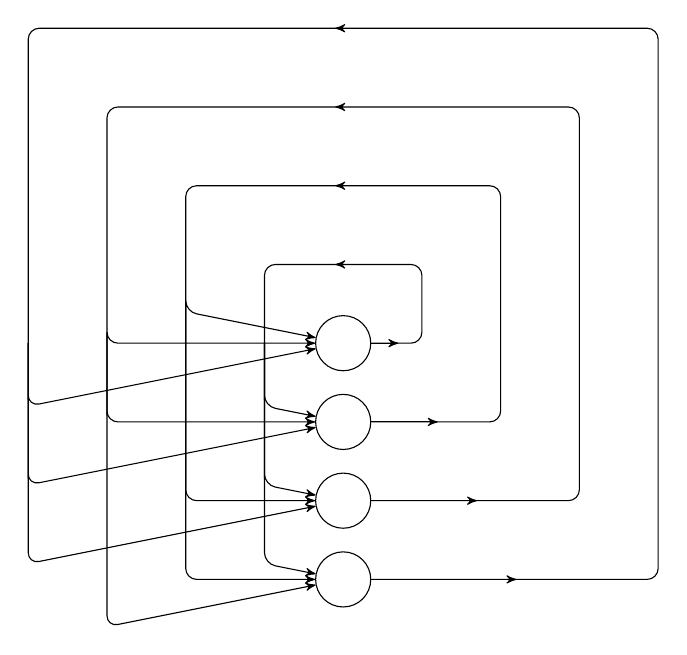
\begin{tikzpicture}[
  neuron/.style={circle,draw,minimum size=7mm},
  on grid,
  > = stealth',
  rounded corners
  ]
  % nodes
  \node[neuron] (a) {};
  \node[neuron,below=of a] (b) {};
  \node[neuron,below=of b] (c) {};
  \node[neuron,below=of c] (d) {};
  % right upper corner of edges
  \coordinate (a1) at ($(a)+(1,1)$);
  \coordinate (b1) at ($(b)+(2,3)$);
  \coordinate (c1) at ($(c)+(3,5)$);
  \coordinate (d1) at ($(d)+(4,7)$);
  % left outermost point of edges
  \coordinate (a2) at ($(a)+(-1,0)$);
  \coordinate (b2) at ($(b)+(-2,1)$);
  \coordinate (c2) at ($(c)+(-3,2)$);
  \coordinate (d2) at ($(d)+(-4,3)$);
  % extra edges
  \draw[->] (a) -| (a1) -| ([yshift=2mm]a2|-d) -- (d);
  \draw[->] (a2) |- ([yshift=2mm]a2|-b) -- (b);
  \draw[->] (a2) |- ([yshift=2mm]a2|-c) -- (c);
  \draw[->] (b) -| (b1) -| (b2|-d) -- (d);
  \draw[->] (b2) |- ([yshift=4mm]b2|-a) -- (a);
  \draw[->] (b2) |- (b2|-c) -- (c);
  \draw[->] (c) -| (c1) -| ([yshift=-6mm]c2|-d) -- (d);
  \draw[->] (c2) |- (c2|-a) -- (a);
  \draw[->] (c2) |- (c2|-b) -- (b);
  \draw[->] (d) -| (d1) -| ([yshift=-8mm]d2|-c) -- (c);
  \draw[->] (d2) |- ([yshift=-8mm]d2|-a) -- (a);
  \draw[->] (d2) |- ([yshift=-8mm]d2|-b) -- (b);
  % arrows
  \draw[->] (a) -- +(0.7,0);
  \draw[->] (b) -- +(1.2,0);
  \draw[->] (c) -- +(1.7,0);
  \draw[->] (d) -- +(2.2,0);
  \draw[->] (a|-a1) -- +(-0.1,0);
  \draw[->] (b|-b1) -- +(-0.1,0);
  \draw[->] (c|-c1) -- +(-0.1,0);
  \draw[->] (d|-d1) -- +(-0.1,0);
\end{tikzpicture}

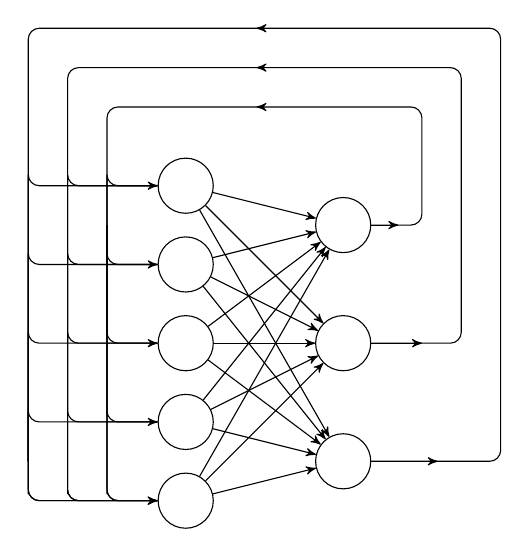
\begin{tikzpicture}[
  neuron/.style={circle,draw,minimum size=7mm},
  on grid,
  > = stealth',
  rounded corners
  ]
  % nodes
  \node[neuron] (a) {};
  \node[neuron,below=of a] (b) {};
  \node[neuron,below=of b] (c) {};
  \node[neuron,below=of c] (d) {};
  \node[neuron,below=of d] (e) {};
  \node[neuron,right=2 of c] (B) {};
  \node[neuron,above=1.5 of B] (A) {};
  \node[neuron,below=1.5 of B] (C) {};
  % right upper corner of edges
  \coordinate (A1) at ($(A)+(1,1.5)$);
  \coordinate (B1) at ($(B)+(1.5,3.5)$);
  \coordinate (C1) at ($(C)+(2,5.5)$);
  % left outermost point of edges
  \coordinate (A2) at ($(A)+(-3,0)$);
  \coordinate (B2) at ($(B)+(-3.5,0)$);
  \coordinate (C2) at ($(C)+(-4,0)$);
  % edges
  \draw[->] (A) -| (A1) -| (A2|-e) -- (e);
  \draw     (B) -| (B1) -| (B2|-e) -- (e);
  \draw     (C) -| (C1) -| (C2|-e) -- (e);
  \foreach \x in {a,b,c,d,e} {
    \draw[->] (A2) |- (A2|-\x) -- (\x);
    \draw     (B2) |- (B2|-\x) -- (\x);
    \draw     (C2) |- (C2|-\x) -- (\x);
  }
  \foreach \x in {a,b,c,d,e} {
    \foreach \y in {A,B,C} {
      \draw[->] (\x) -- (\y);
    }
  }  
  % extra arrows
  \draw[->] (A) -- +(0.7,0);
  \draw[->] (B) -- +(1,0);
  \draw[->] (C) -- +(1.2,0);
  \draw[->] ({(1,0)}|-A1) -- +(-0.1,0);
  \draw[->] ({(1,0)}|-B1) -- +(-0.1,0);
  \draw[->] ({(1,0)}|-C1) -- +(-0.1,0);
\end{tikzpicture}



\tikzset{%
    every neuron/.style={
        circle,
        draw,
        minimum size=1cm
    },
    neuron missing/.style={
        draw=none, fill=none,%<-----------------new
        scale=4,
        text height=0.333cm,
        execute at begin node=\color{black}$\vdots$
    },
}

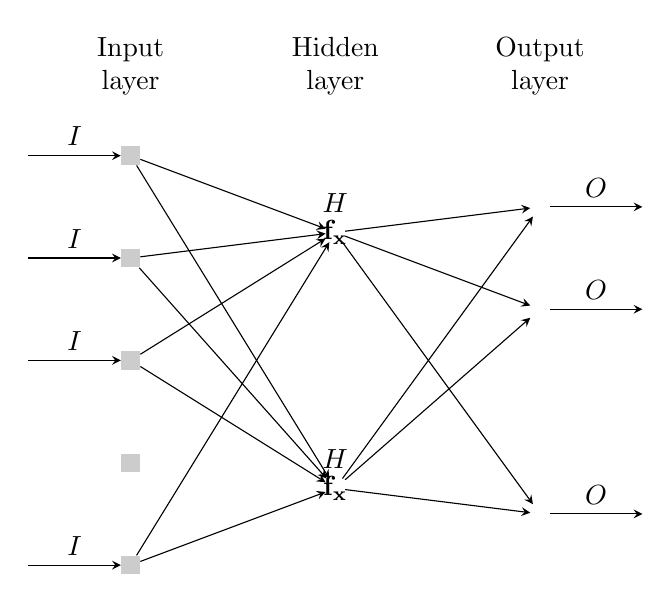
\begin{tikzpicture}[x=1.3cm, y=1.3cm, >=stealth]
    
    \foreach \m/\l [count=\y] in {1,2,3,missing,4}
    \node [fill=black!20, every neuron/.try, neuron \m/.try, ] (input-\m) at (0,2.5-\y) {};%<-----fill=
    
    \foreach \m [count=\y] in {1,missing,2}
    \node [every neuron/.try, neuron \m/.try ] (hidden-\m) at (2,2-\y*1.25) {};
    
    
    \foreach \m [count=\y] in {1,2,missing,3}
    \node [every neuron/.try, neuron \m/.try ] (output-\m) at (4,2.0-\y) {};
    
    \foreach \l [count=\i] in {1,2,3,j}
    \draw [<-] (input-\i) -- ++(-1,0)
    node [above, midway] {$I$};
    
    \foreach \l [count=\i] in {1,k}
    \node [above] at (hidden-\i.north) {$H$};
    
    
    \foreach \l [count=\i] in {1,2,l}
    \draw [->] (output-\i) -- ++(1,0)
    node [above, midway] {$O$};
    
    \foreach \i in {1,...,4}
    \foreach \j in {1,...,2}
    \draw [->] (input-\i) -- (hidden-\j);
    
    \foreach \i in {1,...,2}
    \foreach \j in {1,...,3}
    \draw [->] (hidden-\i) -- (output-\j);
    
    \foreach \l [count=\x from 0] in {Input, Hidden, Output}
    \node [align=center, above] at (\x*2,2) {\l \\ layer};
    \node (nx1) at (hidden-1) {$\mathbf{f_x}$};%<---------------new
    \node (nx2) at (hidden-2) {$\mathbf{f_x}$};%<---------------new
\end{tikzpicture}
\end{document}